\chapter{Implementacja}

\section{Architektura}


\subsection{Struktura interfejsu REST}
Poniższa tabela \ref{tab:rest} prezentuje jakie zapytania mogą być odbierane przez aplikację serwerową. Z racji tego, że w aplikacji wykorzystywane są typy generyczne w klasach kontrolerach urządzeń i komponentów komputera (implementacja \ref{controller_genericDevice} uproszczono tabele by pokazać ogólną formę zapytań. Wszystkie zapytania posiadające "`devices"' w ścieżce umożliwiają alternatywne wywołanie zapytania na podstawie typu sprzętu. Ogólna zasada jest taka aby zastąpić "`devices"' odpowiadającemu typowi sprzętu: "`computers"', "`tablets"', "`other-devices"'. Powoduje to, że zapytanie wykonywane jest przez kontroler tej klasy, a co za tym idzie ma określony typ. Możliwe jest też wykonanie zapytania nie zmieniając ścieżki. Wtedy takie zapytanie wykonywane jest na ogólnym rodzaju sprzętu. Przykładowo "`devices/all"' pobiera wszystkie sprzęty nie zwracając uwagi na typ, natomiast "`computers/all"' pobiera tylko sprzętu typu "`Computer"'. Podobne rozwiązanie wykorzystano w komponentach komputera. Dotyczy to zapytań mających w ścieżce: "`component"'. Tutaj należy zamienić "`component"' na jeden z trzech dostępnych typów komponentu: "`rams"', "`cpus"', "`storages"'. W tym wypadku nie ma możliwości wywołania zapytania zawierającego "`component"'.

\begin{table}[H]
	\centering
\caption{Tabela prezentująca strukturę REST }
\label{tab:rest}
\begin{tabularx}{\linewidth}{|X|X|X|X|}
    \hline
    Ścieżka & Metoda & Parametry & Opis  \\
    \hline \hline
		/devices/all 	& GET & - & Pobranie danych sprzętów na podstawie określonego typu \\
		\hline
		/devices/{id} & GET & identyfikator urządzenia 	& Pobranie danych wszystkich sprzętów\\
    \hline
		/devices/{id}	& DELETE & identyfikator urządzenia 	& Usunięcie sprzętu\\
    \hline
		 /computers/update/id & PUT & Identyfikator sprzętu i zmienione dane sprzętu& aktualizacja danych komputera\\
		\hline
		 /tablets/update/id & PUT & Identyfikator sprzętu i zmienione dane sprzętu& aktualizacja danych tabletu\\
		\hline
		 
		\end{tabularx}
		\end{table}

	\begin{table}[H]
	\centering
	\label{tab:rest}
	\begin{tabularx}{\linewidth}{|X|X|X|X|}
		/other-device/update/id & PUT & Identyfikator sprzętu i zmienione dane sprzętu& aktualizacja danych innego urządzenia\\
		\hline
			 /computers/add & POST	& dane komputera 	& Dodanie nowego komputera	\\
    \hline
		/tablets/add & POST	& dane tabletu & Dodanie nowego urządzenia	\\
    \hline
		/other-device/add & POST	& dane innego urządzenia 	& Dodanie nowego urządzenia	\\
    \hline
		/devices/by-office& GET	& identyfikator biura 	& Pobranie danych sprzętu znajdujących się w biurze\\
    \hline
		/devices/all-ready-to-lottery& GET	& - & Pobranie danych sprzętów które są gotowe do losowania\\
    \hline
		
		/devices/all-ready-to-lottery-by-officeId/id& GET	& Identyfikator biura & Pobranie danych sprzętów które są gotowe do losowania i znajdują się w danym biurze\\
    \hline
		/devices/set-ready-to-lottery/id 		& PUT	& identyfikator sprzętu & Ustawienie gotowości sprzętu do losowania	\\
    \hline
		/devices/set-not-ready-to-lottery/id & PUT	& identyfikator sprzętu & Ustawienie braku gotowości sprzętu do losowania	\\
    \hline
		/devices/set-ordered/id & PUT	& identyfikator sprzętu & Ustawienie statusu sprzętu na dostarczone	do pracownika	\\
    \hline
		/devices/set-not-ordered/id & PUT	& identyfikator sprzętu & Ustawienie statusu sprzętu na dostarczone	do pracownika	\\
    \hline
		/components/all 	& GET & - & Pobranie danych wszystkich procesorów, ram lub dysków pamięci \\
		\hline
		/components/{id} & GET & identyfikator komponentu 	& Pobranie danych procesora, ram lub dysku pamięci\\
    \hline
		/components/{id}	& DELETE & identyfikator komponentu 	& Usunięcie procesora, ram lub dysku pamięci\\
    \hline
		 /components/update/id & PUT & Identyfikator sprzętu i zmienione dane sprzętu& aktualizacja danych komputera\\
		\hline
		 /offices/all	& GET & - & Pobranie wszystkich biur w systemie\\
		\hline
		/users/all	& GET & - & Pobranie wszystkich użytkowników w systemie\\
		\hline
		\end{tabularx}
		\end{table}

		\begin{table}[H]
	\centering
	\label{tab:rest}
	\begin{tabularx}{\linewidth}{|X|X|X|X|}
	 
		
		 /users/all-standard	& GET & -& Pobranie wszystkich użytkowników z rolą pracownik w systemie\\
		\hline
		 /users/id & GET & - & Pobranie użytkownika\\
		\hline
		 /users/id & DELETE & - & Usunięcie użytkownika\\
		\hline
		 /participation/add & POST & identyfikator użytkownika i identyfikator urządzenia & Dodanie uczestnictwa użytkownika w loterii do wybranego sprzętu\\
		\hline
		 /participation/all& POST & - & Wyświetlenie wszystkich uczestników dla każdego sprzętu\\
		\hline
		 /participation/id & DELETE & - & Usunięcie uczestnictwa o zadanym id\\
		\hline
		 /participation/delete-by-user\_id-and-device\_id& DELETE & identyfikator użytkownika i identyfikator sprzętu & Usunięcie uczestnictwa spełniającego zadane kryteria\\
		\hline
		 /participation/all-wins& GET & - & Wyświetlenie wszystkich zwycięskich uczestników\\
		\hline
		 /participation/user-lottery-history/id & GET& identyfikator użytkownika & Wyświetlenie historii uczestnictwa użytkownika o zadanym id\\
		\hline
		 /participation/user-win-history/id & GET& identyfikator użytkownika & Wyświetlenie historii zwycięstw użytkownika o zadanym id\\
		\hline
		 /participation/user-lose-history/id & GET& identyfikator użytkownika & Wyświetlenie historii porażek użytkownika o zadanym id\\
		\hline
		 /participation/user-pending-lottery/id & GET& identyfikator użytkownika & Wyświetlenie uczestnictwa które czeka na losowanie\\
		\hline
		 /participation/device-participation/id& GET& identyfikator urządzenia & Wyświetlenie wszystkich użytkowników zapisanych na losowaniu urządzenia o zadanym id\\
		\hline
		 /participation/check-if-user-in-lottery& GET& identyfikator urządzenia i identyfikator użytkownika& Sprawdzenie czy użytkownik bierze udział w losowaniu\\
		\hline
		 /participation/select-random-winner/id& GET& identyfikator urządzenia& Losowanie zwycięzcy loterii dla urządzenia o zadanym id\\
		\hline
\end{tabularx}
\end{table}



\section{Aplikacja serwerowa}
Do zarządzania danymi wykorzystywana jest aplikacja serwerowa. Przetwarza ona żądania aplikacji klienckiej. Dostarcza ona funkcjonalność uwierzytelniania i autoryzacji. W wyniku zapytań wysłanych przez aplikację kliencką wyświetlane są w aplikacji odpowiednie dane. Możliwe jest też dodawanie i usuwanie odpowiednich rekordów. Implementacja odbywa się z wykorzystywaniem języka Java z frameworkami Spring oraz Hibernate \ref{tab:zestawienie_narzędzi} Graficzną reprezentacje struktury projektu aplikacji serwerowej pokazano na rysunku \ref{backend_struktura:label}

\subsection{Struktura projektu}
Ścieżka pakietowa wykorzystana jest odwróconą ścieżką domenową Politechniki Wrocławskiej oraz nazwy projektu: pl.edu.pwr.computermanagamenttool. Następnie pakiety które są dołączone do tej ścieżki odpowiadają funkcjom które pełnią klasy. Wyróżnia się tutaj pakiety:
\begin{itemize}
\item pl.edu.pwr.computermanagementtool - pakiet ogólny przechowywujący pozostałe pakiety. Klasa ComputerManagementToolApplication posiada metodę Main odpowiedzialną za uruchomienie aplikacji. Klasa JacksonConfig jest konfiguracją odpowiedzialną za serializacje formatu JSON. Natomiast klasa PasswordEncoderUtil jest odpowiedzialna za szyfrowanie haseł użytkowników korzystających z systemu.
\item controller - pakiet przechowujący w sobie klasy kontrolerów odpowiedzialne za wykonywanie zapytań aplikacji za pomocą interfejsu REST
\item dto - pakiet który jest odpowiedzialny za przechowywanie klas służących do przechowywania danych i ułatwiania ich przesyłania między różnymi częściami systemu. Wykorzystywany jest w klasach kontrolera.
\item entity - pakiet przechowujący definicje encji reprezentowanych w bazie danych
\item repository - pakiet przechowujący repozytoria służące do komunikacji z bazą danych.
\item service - pakiet przechowujący serwisy które są odpowiedzialne za warstwę logiki biznesowej w systemie
\end{itemize}


\begin{figure}[htb]
  \centering
	\begin{tabular}{@{}lll@{}}
	a) & b) & c) \\
  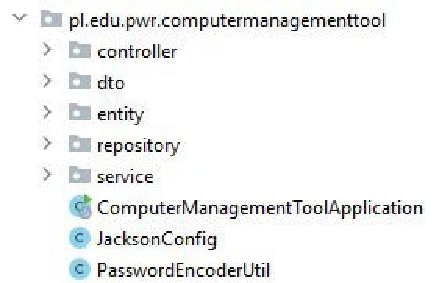
\includegraphics[width=0.3\textwidth]{rys05/ogolne.pdf} & 
	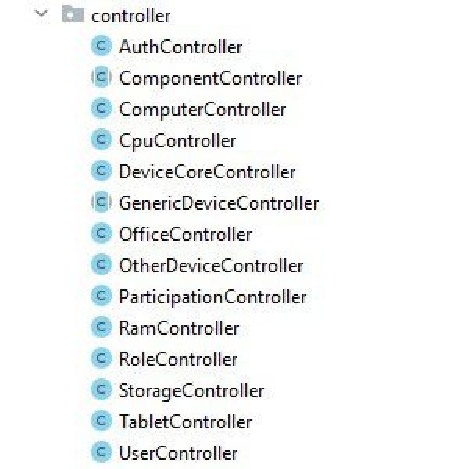
\includegraphics[width=0.3\textwidth]{rys05/controller.pdf} &
	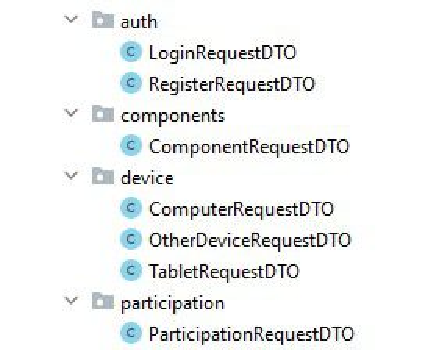
\includegraphics[width=0.3\textwidth]{rys05/dto.pdf} \\

	d) & e) & f) \\
	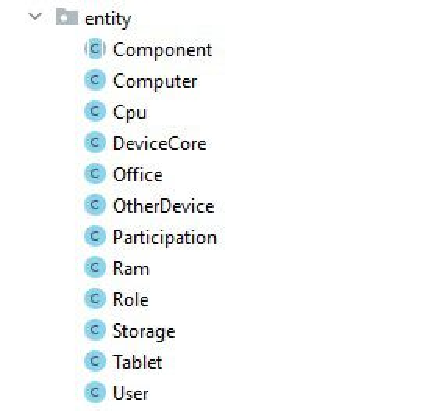
\includegraphics[width=0.3\textwidth]{rys05/entity.pdf} &
	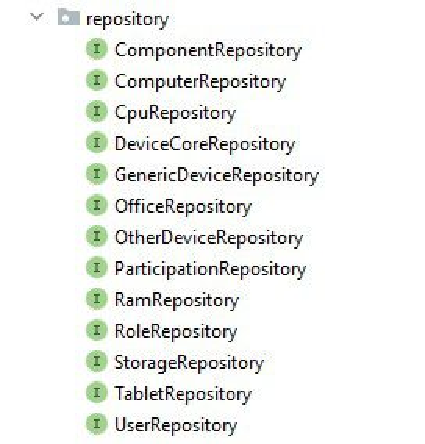
\includegraphics[width=0.3\textwidth]{rys05/repository.pdf} &
	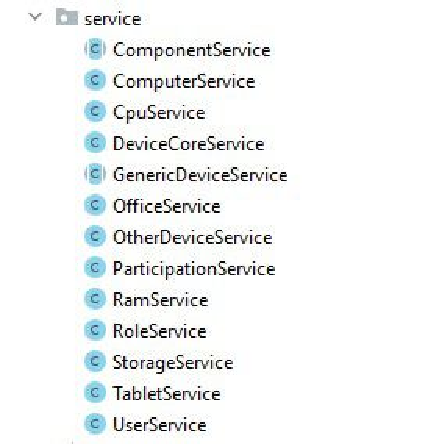
\includegraphics[width=0.3\textwidth]{rys05/service.pdf}
	\end{tabular}
  \caption{Struktura projektu a) ogólna struktura, b) kontrolery, c) data transfer object, d) encje, e) repozytoria, f) serwisy}
  \label{backend_struktura:label}
\end{figure}

\newpage
\subsection{Fragmenty implementacji}
\subsubsection {Fragment kodu klas encji wykorzystującej schemat dziedziczenia}

\begin{lstlisting}[language=Java, style=JavaStyle, caption={Klasa nadrzędna reprezentująca rdzeń sprzętu: DeviceCore}, label={entity_deviceCore}]
@Entity
@Table(name = "device_core")
@Inheritance(strategy = InheritanceType.TABLE_PER_CLASS)
public class DeviceCore {
    @Id
    @GeneratedValue(strategy = GenerationType.TABLE)
    @Column(name = "id", nullable = false)
    private Integer id;

    @Column(name = "device_type", length = 50)
    private String deviceType;

    @Column(name = "device_name", length = 50)
    private String deviceName;
		
		// Pozostała część klasy

\end{lstlisting}
W linii 3 listingu klasy DeviceCore \ref{entity_deviceCore} określono schemat dziedziczenia TABLE\_PER\_CLASS. O sposobie dziedziczenia napisano w podrozdziale \ref{dzedziczenie_hibernate:label}. Linia 3 określa strategie generowania klucza. Hibernate tworzy wtedy specjalną tabelę w bazie danych która odpowiedzialna jest za przechowywanie unikalnych kluczy głownych dla encji sprzętu w aplikacji. W listingu kodu \ref{entity_computer} nie trzeba wtedy definować klucza.

\begin{lstlisting}[language=Java, style=JavaStyle,  caption={Klasa potomna: Computer, reprezentująca komputer}, label={entity_computer}]
@Entity
@Table(name = "computer")
public class Computer extends DeviceCore{

    public static final String DEVICE_TYPE = "COMPUTER";
    @Column(name = "serial_number", length = 50)
    private String serialNumber;

    @Column(name = "operating_system", length = 50)
    private String operatingSystem;

    @Column(name = "battery_life", length = 50)
    private String batteryLife;
		
		// Pozostała część klasy
\end{lstlisting}
W linii 3 określone zostało dziedziczenie po klasie nadrzędnej reprezentującej rdzeń sprzętu. Pola które należy określić w tej klasie są unikalnymi polami tabeli computer. W linii 4 istnieje statyczna zmienna DEVICE\_TYPE która pomaga określić jakiego rodzaju dany sprzęt. Wykorzystywane jest to w aplikacji klienckiej.


\subsubsection{Przykład kodu repozytorium dla urządzeń dziedziczącym po rdzeniu sprzętu}
Repozytorium sprzętu komputerowego zostało napisane z użyciem wyrażeń generycznych. Wykorzystanie ich przyczynia się do uproszczenia kodu oraz łatwiejszej jego rozbudowy.

\begin{lstlisting}[language=Java, style=JavaStyle,  caption={Generyczne repozytorium sprzętu komputerowego:  GenericDeviceRepository}, label={repo_genericDevice}]
@NoRepositoryBean
public interface GenericDeviceRepository<T extends DeviceCore> extends JpaRepository<T, Integer> {
    
    List<T> findAllByReadyToLotteryIsTrue();
    List<T> findAllByOfficeId(int officeId);
}
\end{lstlisting}

W lini 1 adnotacja @NoRepositoryBean jest używana do oznaczenia interfejsów które nie mają mieć swojej instancji. Oznacza to, że nie jest on przeznaczony do utworzenia instancji repozytorium w trakcie uruchomiania aplikacji. W linii 4 i 5 poprzez zdefiniowanie metody możliwe jest wykonanie konkretego zapytania SQL do bazy danych. Z racji, że klasy sprzętu komputerowego mają zbliżone funkcjonalności nie trzeba dostarczać tych samych interfejsów we wszystkich repozytoriach tylko zastosować schemat dziedziczenia.

\subsubsection{Fragmenty implementacji klasy kontrolerów sprzętu}

\begin{lstlisting}[language=Java, style=JavaStyle,  caption={Klasa nadrzędna kontrolera sprzętu: GenericDeviceController}, label={controller_genericDevice}]
public abstract class GenericDeviceController<T extends DeviceCore> {

    protected final GenericDeviceService<T> genericDeviceService;
    protected final GenericDeviceRepository<T> genericRepository;

    protected GenericDeviceController(GenericDeviceService<T> genericDeviceService, GenericDeviceRepository<T> genericRepository) {
        this.genericDeviceService = genericDeviceService;
        this.genericRepository = genericRepository;
    }

    @GetMapping("/{id}")
    @CrossOrigin(origins = "*")
    T getOneBasicDevice(@PathVariable int id){
        return genericDeviceService.getDeviceById(id);
    }

    @GetMapping("/all")
    @CrossOrigin(origins = "*")
    List<T> getAllBasicDevices(){
        return genericDeviceService.getAllDevices();
    }

    @GetMapping("/all-ready-to-lottery")
    @CrossOrigin(origins = "*")
    List<T> getAllReadyToLotteryDevice(){
        return genericDeviceService.getAllReadyToLotteryDevices();
    }
		
		// Pozostała część klasy
		
		@PutMapping("/set-ready-to-lottery/{id}")
    @CrossOrigin(origins = "*")
    public ResponseEntity<T> setReadyToLottery(@PathVariable int id){
        try{
            T updatedBasicDevice = genericDeviceService.setReadyToLottery(id);
            return new ResponseEntity<>(updatedBasicDevice, HttpStatus.OK);
        } catch (RuntimeException e){
            return new ResponseEntity<>(HttpStatus.NOT_FOUND);
        }
    }
		
		// Pozostała część klasy
		
\end{lstlisting}

Kontrolery pełnią istotną funkcje w systemie. Umożliwiają one definiowanie zapytań REST które będą wysyłane do serwera. Wykorzystując abstrakcje oraz wyrażenia generyczne możliwe jest wykonanie niektórych requestów bez konieczności ich implementacji w klasach potomnych.


\begin{lstlisting}[language=Java, style=JavaStyle,  caption={Klasa potomna reprezentująca ogólną postać sprzętu}, label={controller_device}]
@RestController
@RequestMapping("/devices")
public class DeviceCoreController extends GenericDeviceController<DeviceCore>{

    protected DeviceCoreController(DeviceCoreService deviceCoreService, GenericDeviceRepository<DeviceCore> genericRepository) {
        super(deviceCoreService, genericRepository);
    }
}
\end{lstlisting}

Powyższa klasa w listingu kodu \ref{controller_device} nie posiada własnych metod. Umożliwia jednak wykonywanie ogólnych operacji dotyczących sprzętu. Możliwe jest między innymi pobranie informacji dotyczące sprzętu bez względu na jego typ co idealanie obrazuje test **referencja do zapytania w postmanie**


\subsubsection{Fragmenty implementacji klas serwisów sprzętu}


\begin{lstlisting}[language=Java, style=JavaStyle,  caption={Klasa nadrzędna serwisu sprzętu GenericDeviceService}, label={service_tablet}]

public abstract class GenericDeviceService<T extends DeviceCore> {

    protected final GenericDeviceRepository<T> genericDeviceRepository;
    protected final OfficeRepository officeRepository;

    public GenericDeviceService(GenericDeviceRepository<T> genericRepository, OfficeRepository officeRepository) {
        this.genericDeviceRepository = genericRepository;
        this.officeRepository = officeRepository;
    }

    public T getDeviceById(int id) {
        Optional<T> basicDeviceOptional = genericDeviceRepository.findById(id);
        return basicDeviceOptional.orElseThrow(()-> new RuntimeException("Device not found with id: " + id));
    }

    public List<T> getAllDevices() {
        return genericDeviceRepository.findAll();
    }
		// Pozostała część klasy

protected DeviceCore addDevice(Class<? extends DeviceCore> deviceClass, String deviceName, Double price, String description, Integer age, Boolean readyToSell, Integer officeId) {

        if(officeId == null){
            throw new RuntimeException("Office required");
        }
        Optional<Office> officeOptional = officeRepository.findById(officeId);
        Office office = officeOptional.orElseThrow(() -> new RuntimeException("Office not found with id: " + officeId));

        DeviceCore deviceCore;
        try {
            deviceCore = deviceClass.getDeclaredConstructor().newInstance();
        } catch (InstantiationException | IllegalAccessException | NoSuchMethodException | InvocationTargetException e) {
            throw new RuntimeException("Error creating device", e);
        }

        deviceCore.setDeviceName(deviceName);
        deviceCore.setPrice(price);
        deviceCore.setDescription(description);
        deviceCore.setAge(age);
        deviceCore.setReadyToSell(readyToSell);
        deviceCore.setOffice(office);

        return deviceCore;
    }
		
		// Pozostała część klasy

\end{lstlisting}
Serwisy są odpowiedzialne za warstwe logiki biznesowej systemu. W linii 12 widnieje metoda która pozwala na pobranie sprzętu. W linii 17 natomiast jest możliwe pobranie wszystkich sprzętów. Odbywa się to przy pomocy parametryzowanych typów danych T. Metoda zdefiniowana w linii 22 pozwala uprościć dodawanie sprzętu, implementując część logiki ustawiając parametry charakterystyczne dla rdzenia sprzętu. Jednak aby utworzyć odpowiedni typ niezbędne jest określenie jakiego typu będzie dodawane urządzenie, Dlatego w linii 22 metoda jako parametr przyjmuje Class<? extends DeviceCore> który oznacza typ aplikacji. Tak zdefiniowana metoda może zostać użyta do dodania sprzętu w kalsach potomnych co pokazano w listingu \ref{service_tablet}

\begin{lstlisting}[language=Java, style=JavaStyle,  caption={Klasa potomna serwisu tabletu: TabletService }, label={service_tablet}]

@Service
public class TabletService extends GenericDeviceService<Tablet>{

    public TabletService(TabletRepository tabletRepository, OfficeRepository officeRepository){
        super(tabletRepository, officeRepository);
    }

    public Tablet addTablet(String deviceName, Double price, String description,
                            Integer age, String officeAddress,
                            String screenSize, String operatingSystem, String batteryLife){

        Tablet tablet = (Tablet) addDevice(Tablet.class, deviceName, price, description,
                                                                age, officeAddress);

        tablet.setScreenSize(screenSize);
        tablet.setOperatingSystem(operatingSystem);
        tablet.setDeviceType(Tablet.DEVICE_TYPE);
        tablet.setBatteryLife(batteryLife);

        return genericDeviceRepository.save(tablet);
    }
		\\pozostała część klasy
\end{lstlisting}

Serwis klasy TabletService dziedziczy i parametryzuje metody klasy GenericDeviceService. Wykorzystuje on w linii 13 metode klasy nadrzędnej co upraszaq implementacje metody dodającej sprzęt(linia 9)



\section {Aplikacja kliencka}
%TODO wstęp

\subsection{Struktura projektu}


\subsection{Fragmenty implementacji}
\subsubsection{Widoki aplikacji}
%TODO opisy scieżek w aplikacji
\subsubsection{Renderowanie danych w tabeli}

\subsection{Instrukcja użytkowania}
\subsubsection{Logowanie i rejestracja}

\subsubsection{Administrator}
\subsubsection{Pracownik}



